\documentclass[a4paper,12pt]{article}
\usepackage{amsmath, amssymb}
\usepackage{graphicx}
\usepackage{multirow}
% \usepackage[UTF8]{ctex} % use ctex enable Chinese

% -------------------------------------------
\begin{document}

% title -------------------------------------
\title{My First Document}
\author{Yichen Mo}
\date{\today}
\maketitle

% toc ---------------------------------------
\pagenumbering{roman} % page number for toc
\tableofcontents
\newpage
\pagenumbering{arabic} % page number for rest article


% content -----------------------------------
\section{Introduction}
This is the introduction.

\section{Related Works}
Former works.\cite{Birdetal2001}

\section{Methods}

\subsection{Stage 1}
The first part of the methods.


% equation ----------------------------------
These are labeled equations
\begin{equation}
    e = mc^2
\end{equation}

\begin{equation}
    \pi = \frac{c}{d}
\end{equation}

This is no label equation
\begin{equation*}
    \pi = \frac{c}{d}
\end{equation*}

\subsection{Stage 2}
The second part of the methods. See the table \ref{table:1}

% table -------------------------------------
\begin{table}[h!]
    \centering
    \caption{Table to test captions and labels} % table name usually at the top
    \label{table:1}
    \begin{tabular}{ l | c c c }

        \multirow{2}{4em}{City} & \multicolumn{3}{l}{Year} \\ 
        \cline{2-4}
                           & 2006 & 2007 & 2008 \\
        \hline
        London & 45789 & 45628 & 48922 \\
        Berlin & 29392 & 23912 & 49293 \\
        Paris & 38281 & 29312 & 29341 \\
    \end{tabular}
\end{table}

\section{Results}
Here are my results. Show in the figure \ref{resulttest}

% figures -----------------------------------
\begin{figure}[ht!] % h-here t-top b-bottom p-new page !-force
    \centering
    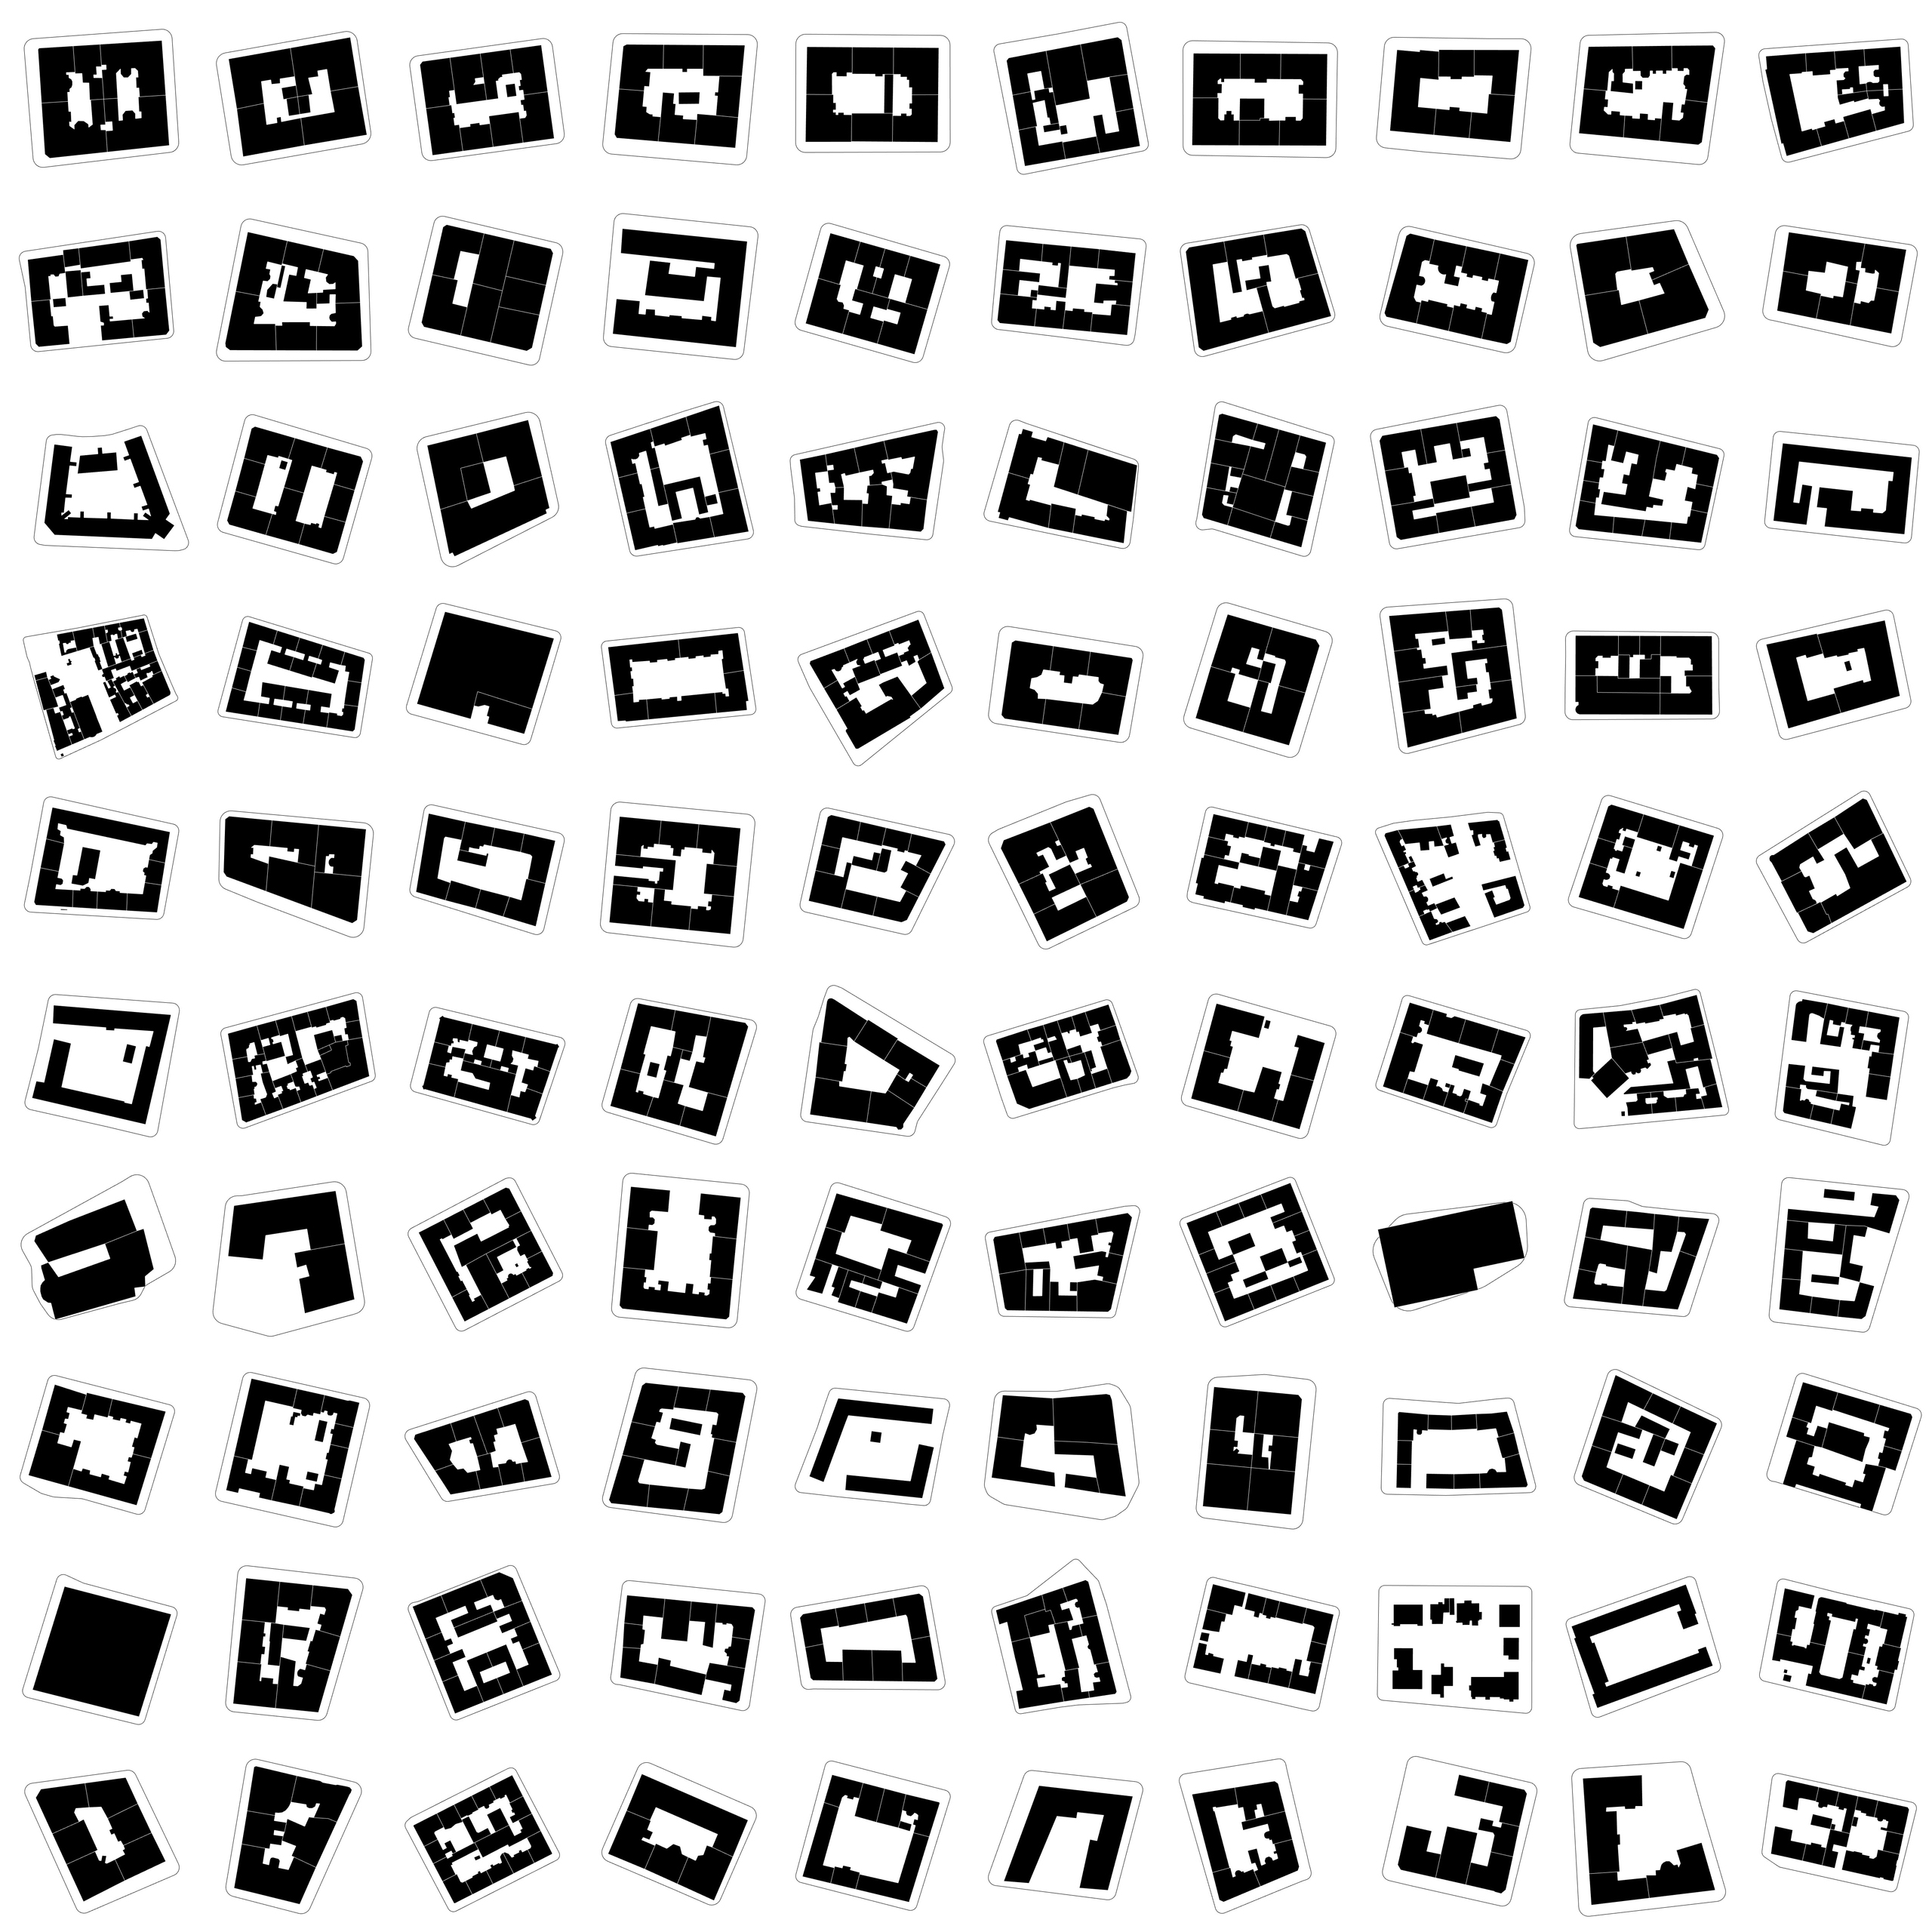
\includegraphics[width=1\textwidth]{images/result.jpg}
    \caption{My test image}
    \label{resulttest} % reference
\end{figure}

% reference ---------------------------------
\newpage
% \bibliographystyle{abbrv} % use abbrv. author name
\bibliographystyle{plain} % use numbered list [1]
% \bibliographystyle{unsrt} % unsort reference (in paper)
% \bibliographystyle{alpha} % use author name list [BSB01]
\bibliography{template}

% list of figures ---------------------------
\newpage
\listoffigures

\end{document}
